\chapter{Porovnání programů}
\label{chap:diskuze}

V \myref{kapitole}{chap:programovani} jsem programoval algoritmy, které jsem uvedl v teoretické části. Programy jsem zkoušel na náhodně generovaných bodech a také jsem je zkontroloval jiným algoritmem, který zkouší úplně všechny možnosti. Podle testů, které jsem provedl, by měly fungovat správně. Může se ale stát, že Python nebo nějaké knihovny, které používám, se změní a poté se bude muset program upravit. 

% Udělat graf s porovnáním čas / počet bodů a u nD něco jako čas při počtu bodů a při jaké dimenzi.

\begin{figure}
\centering
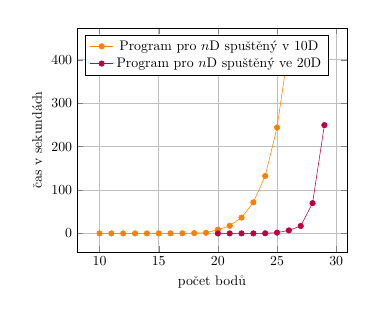
\begin{tikzpicture}[scale=0.5]
    \begin{axis}[
        xlabel={počet bodů},
        ylabel={čas v sekundách},
        legend pos=north west,
        grid=both,
    ]
    
    % Function 4
    \addplot[color=orange, mark=*] coordinates {
        (10,0.0004)
        (11,0.0021)
        (12,0.0008)
        (13,0.0027)
        (14,0.0110)
        (15,0.0485)
        (16,0.1121)
        (17,0.2974)
        (18,0.7327)
        (19,1.5065)
        (20,8.580572)
        (21,17.67404)
        (22,36.42449)
        (23,71.50185)
        (24, 132.2238)
        (25, 243.9930)
        (26, 430.1611)
    };
    
    % Function 5
    \addplot[color=purple, mark=*] coordinates {
        (20,0.0015933)
        (21,0.0019776)
        (22,0.0052187)
        (23,0.0354709)
        (24,0.2808427)
        (25,1.8337924)
        (26,6.9350697)
        (27, 17.14)
        (28, 69.68)
        (29, 249.38)

    };
    
    \legend{Program pro $n$D spuštěný v 10D, Program pro $n$D spuštěný ve 20D}
    \end{axis}
\end{tikzpicture}
\caption{Three simple graphs}
\label{obr:three graphs}
\end{figure}